The Rubik's Cube community has developed a standardised notation to efficiently represent moves.
Each face of the cube is assigned a letter, and rotations of faces are represented by their corresponding letters followed by some modifiers.
\begin{itemize}
	\item A single letter (Eg. \alg{F}) means the face must be turned clockwise by 90\degree .
	\item A letter followed by a prime (Eg. \alg{R'}) means the face must be turned \emph{counter}-clockwise by 90\degree .
	\item A letter followed by `2' (Eg. \alg{U2}) means the face should be turned 180\degree . In this case, the direction of rotation does not matter.
\end{itemize}
Note that these moves are always relative to the face that the solver is looking at; see \figref{notation}.
\begin{figure}[h]
	\centering
	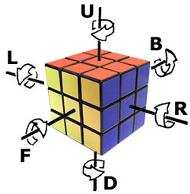
\includegraphics[width=.2\textwidth]{notation.jpg}
	\caption{Move notation}\label{fig:notation}
\end{figure}
These individual moves can be concatenated to produce move sequences, such as the very commonly used `corner algorithm', \alg{FRUR'U'F'}. Giving such commonly used algorithms names allows one to recognise algorithms that one has already learnt.